\documentclass[12pt]{ctexart}
\usepackage{amsmath,graphicx,textcomp,subfigure,indentfirst,ctex,color,float}
\title{Lecture 5}
\author{赵思逸}

\date{\today}
\newcommand{\new}[1]{\textcolor{blue}{#1}}

\newcommand{\refeq}[1]{式~(\ref{#1})}
\newcommand{\reffig}[1]{图~(\ref{#1})}


\begin{document}

\maketitle

\section{弗里德曼(Friedmann)方程}

广义相对论给出爱因斯坦引力场方程
\begin{equation} \label{eq:field}
    G_{\mu \nu} = 8 \pi G T_{\mu \nu}
\end{equation}
该公式左边是爱因斯坦张量(Einstein tensor),表示时空的几何性质,右边的$T_{\mu\nu}$是能动量张量(Energy-momentum tensor),由密度$\rho$、压强$P$决定,描述物质的分布。
引力场方程告诉我们:物质分布决定时空几何。

由\refeq{eq:field}可以得到关于$a(t)$的方程,即弗里德曼(Friedmann)方程。
本课不做推导,直接给出结论。

我们考虑的物质是宇宙中的理想流体,用密度$\rho$和压强$P$描述,它们决定时空几何 $a(t)$ 和 $K$ 如何演化,即 Friedmann 方程
\begin{eqnarray}
    &&\dot{a}^2+K = \frac{8}{3} \pi G \rho a^2 \label{eq:adot} \\
    &&\frac{\ddot{a}}{a} = -\frac{4}{3} \pi G (\rho + 3P) \label{eq:addot}
\end{eqnarray}
其中$G$是牛顿引力常数,$\rho$是宇宙中物质的密度, $P$是宇宙中物质的压强。 
我们使用了自然单位制中的光速 $c=1$,\refeq{eq:addot}中的量纲在补齐$c$之后统一,$[P]=[\rho] \times [c^2]$ 。


由\refeq{eq:adot}可推出哈勃参数的表达式$H(a)=\sqrt{\frac{8}{3}\pi G \rho(a)-\frac{K}{a^2}}$


下面我们考虑\refeq{eq:adot}和\refeq{eq:addot}的关系。对\refeq{eq:adot}求时间导数
\begin{eqnarray}
    \frac{d(1)}{dt} : \qquad 2\dot{a}\ddot{a} = \frac{8}{3} \pi G (\dot{\rho} a^2 + 2\rho a \dot{a})
\end{eqnarray}
代入\refeq{eq:addot}得到
\begin{eqnarray}
    \dot{\rho} = -3\frac{\dot{a}}{a}(\rho+P) \label{eq:EnergyCon}
\end{eqnarray}

\refeq{eq:EnergyCon}就是能量守恒方程。在\refeq{eq:EnergyCon}左右乘上$a^3 V_\text{com}$得到$\frac{d}{dt}(V\rho) = -P\frac{dV}{dt}$就可以看出表示能量守恒。

\section{宇宙中的物质}

\subsection{辐射(Radiation)}

辐射是指极端相对论性的物质,热运动的动能远远大于静质量,即 $m_0 c^2 \ll k_B T$。
例如光子(静质量为0)、中微子(静质量很小)、高温电子气体(静质量 $0.5 \mathrm{MeV} \ll k_B T$)。

量子统计给出辐射的状态方程为 $P=\frac{1}{3}\rho$。
代入\refeq{eq:EnergyCon}得到 $\frac{d\rho}{\rho} = -4\frac{da}{a}$,因此 
\begin{equation}
    \rho_R\propto a^{-4}.
\end{equation}

从物理图像上可以理解为$\rho_R = \frac{\Delta N \hbar\nu }{\Delta V}\propto a^{-4}$, 因为$\Delta N$不变,体积膨胀 $\Delta V \propto a^{3}$ 且 波长被拉长 $\nu \propto a^{-1}$ 。

\subsection{冷物质(Matter)}

冷物质是指非相对论性物质,热运动的动能相比静质量可以忽略,即 $m_0 c^2 \gg k_B T$。
例如冷重子物质、冷暗物质、低温电子气体(静质量 $0.5 \mathrm{MeV} \gg k_B T$)。

% 理想气体状态方程 $PV=NRT$,压强 $P$ 与温度相关,远小于 $\rho$, 即 
冷物质的状态方程为 $P=0$。
代入\refeq{eq:EnergyCon}得到 $\frac{d\rho}{\rho} = -3\frac{da}{a}$,因此
\begin{equation}
    \rho_M\propto a^{-3}.
\end{equation} 

从物理图像上可以理解为$\rho_M = \frac{m_0 \Delta N}{\Delta V}\propto a^{-3}$,因为$\Delta N$不变,体积膨胀 $\Delta V \propto a^{3}$ 。

\subsection{真空能(Vacuum energy)}

真空能就是宇宙学常数,是暗能量的一种。

真空能密度不变 $\rho_\Lambda=const.$,膨胀时外界对内部做功,能量守恒$\Delta E = -\rho_\Lambda \Delta V = P_\Lambda \Delta V$,即真空能的状态方程为 $P_\Lambda = -\rho_\Lambda$。 真空能具有负压 $P_\Lambda < 0 $.

\subsection{一般情况}

一般情况下的状态方程写作$P=w\rho$,将状态方程代入\refeq{eq:EnergyCon}得到
\begin{eqnarray}
    \dot{\rho} &=& -3(1+w) \frac{\dot{a}}{a} \rho 
    \\ \rho &\propto& a^{-3-3w}
\end{eqnarray}

对于我们上面讨论过的三种物质
\begin{table}[htb]
    \centering
    \begin{tabular}{|c|c|c|}
    \hline
    辐射  & $\rho_R\propto a^{-4}$ & $w=1/3$ \\ \hline
    冷物质 & $\rho_M\propto a^{-3}$ & $w=0$   \\ \hline
    真空能 & $\rho_\Lambda=const.$  & $w=-1$  \\ \hline
    \end{tabular}
\end{table}

真空能密度不随宇宙膨胀变化,辐射和冷物质的密度都会随宇宙膨胀而下降,辐射下降得更快。这三种物质的密度随红移的演化如 \reffig{fig:matters-a} 所示。

\begin{figure}[!hbtp]
    \centering
    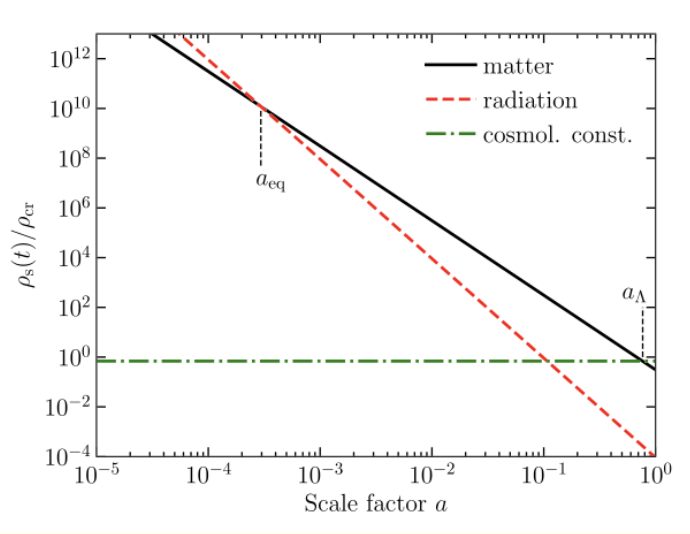
\includegraphics[width=0.8\textwidth]{figures/matters-a.png}
    \caption{辐射、冷物质和真空能密度随尺度因子的演化。Figure 1.3 of Dodelson \& Schmidt, Modern Cosmology, 2nd Edition.}
    \label{fig:matters-a}
\end{figure}

\section{宇宙的演化}

\subsection{平坦宇宙}
考虑平坦宇宙 $K=0$ ,\refeq{eq:adot}变成
\begin{eqnarray}
    \dot{a}^2 = \frac{8}{3} \pi G \rho a^2 \propto \rho a^2
\end{eqnarray} 

\begin{itemize}
    \item 辐射为主时,代入$\rho_R\propto a^{-4}$,得到$a\propto t^{1/2}$。$H=\frac{da/dt}{a}=\frac{1}{2t}$ ,宇宙的年龄 $t_0=\frac{1}{2H_0}$,其中$H_0^{-1}= 9.778 h^{-1} \mathrm{Gyr}$,可以作为对宇宙年龄的粗略估计(实际的宇宙年龄需要考虑$H_0^{-1}$前面的系数)。
    \item 冷物质为主时,代入$\rho_M\propto a^{-3}$,得到$a\propto t^{2/3}$,比辐射为主的宇宙膨胀快。宇宙的年龄 $t_0=\frac{2}{3H_0}$。
    \item 真空能为主时,代入$\rho_\Lambda =const.$,得到$a\propto e^{Ht}$,随e指数加速膨胀。
\end{itemize}

\subsection{冷物质主导的非平坦宇宙}
考虑 $K\neq 0$,冷物质为主的宇宙。由$\rho_M\propto a^{-3}$得到密度$\rho a^3 = \rho_0 a^3_0$,下标0表示今天的量。\refeq{eq:adot}变成
\begin{eqnarray}
    \dot{a}^2 + K = \frac{8}{3} \pi G \rho_0 a_0^3/a 
\end{eqnarray} 
由此得到
\begin{eqnarray}
    \dot{a}&=&\sqrt{\frac{8 \pi G \rho_{0} a_{0}^{3}}{3 a}-K} \\
    d t&=&\frac{d a}{\sqrt{\frac{8}{3} \pi G \frac{\rho_{0} a_{0}^{3}}{a}-K}} \label{eq:dt}
\end{eqnarray}
将 $H_0^2+\frac{K}{a_0^2}=\frac{8}{3}\pi G \rho_0$  代入 \refeq{eq:dt},得到
\begin{equation}
    d t=\frac{d a}{\sqrt{\left(H_{0}^{2}+\frac{K}{a_{0}^{2}}\right) \frac{a_{0}^{3}}{a}-K}}=\frac{d x}{H_{0}} \sqrt{\frac{x}{1+\frac{K}{a_{0}^{2} H_{0}^{2}}(1-x)}} \label{eq:dt-dx}
\end{equation}
其中 $x=a/a_0$,积分得到 $t$ 与 $a$ 的关系 
\begin{equation}
    t=\frac{1}{H_{0}} \int_{0}^{a/a_{0}} \sqrt{\frac{x}{1+\frac{K}{a_{0}^{2} H_{0}^{2}}(1-x)}} d x
\end{equation}

考虑$K=+1$。定义 $\Omega_K \equiv -\frac{K}{a_0^2 H_0^2}$ , $K=+1$时,$\Omega_K <0$ 。
令 $x=\frac{a}{a_{0}}=\frac{1}{2}\left(\frac{1+| \Omega_{K} \mid}{\left|\Omega_{K}\right|}\right)(1-\cos \alpha)$,\refeq{eq:dt-dx}变成
\begin{equation}
    d t=\frac{d x}{H_{0}} \sqrt{\frac{x}{1+\left|\Omega_{K}\right|(1-x)}}=\frac{1}{2 H_{0}} \frac{\left(1+\left|\Omega_{K}\right|\right)}{\left|\Omega_{K}\right|^{3 / 2}} \sin \alpha d \alpha \sqrt{\frac{1-\cos \alpha}{1+ \cos  \alpha}}
\end{equation}
积分得到
\begin{equation}
    t=\frac{1}{2 H_{0}} \frac{\left(1+\left|\Omega_{K}\right|\right)}{\left|\Omega_{K}\right|^{3 / 2}}(\alpha-\sin \alpha)
\end{equation}

\begin{figure}[!hbtp]
    \centering
    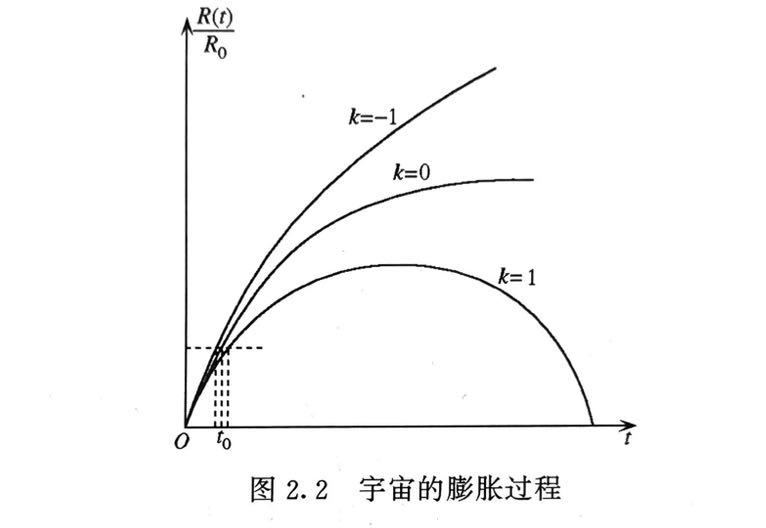
\includegraphics[width=0.8\textwidth]{figures/expansion_k.jpg}
    \caption{冷物质主导下的宇宙膨胀过程,图中$R$是我们的尺度因子$a$。\\ 图源:俞允强《热大爆炸宇宙学》}
    \label{fig:expansion_k}
\end{figure}


\subsection{临界密度}
定义宇宙的临界密度
\begin{equation}
    \rho_\text{crit} \equiv \frac{3H_0^2}{8\pi G} \simeq 1.878\times 10^{-29} h^2 \mathrm{~g~cm^{-3}}
\end{equation}
它是今天平直宇宙所要求的物质密度。


为了满足\refeq{eq:adot},
\begin{itemize}
    \item 若$\rho=\rho_\text{crit}$,则$K=0$。
    \item 若$\rho>\rho_\text{crit}$,则$K=+1$。
    \item 若$\rho<\rho_\text{crit}$,则$K=-1$。
\end{itemize}

\subsection{一般情况下的弗里德曼方程}

考虑最一般的情况

\begin{eqnarray}
    \rho(a) &=& \rho_R(a) + \rho_M(a) + \rho_\Lambda (a) \label{eq:rho}
    \\ &=& \rho_{R,0}\left(\frac{a}{a_0}\right)^{-4} + \rho_{M,0}\left(\frac{a}{a_0}\right)^{-3}  + \rho_{\Lambda,0}     
\end{eqnarray}

定义$\Omega_i$是今天各物质成分在临界密度中的占比,$\Omega_R\equiv\frac{\rho_{R,0}}{\rho_\text{crit}}$, $\Omega_M\equiv\frac{\rho_{M,0}}{\rho_\text{crit}}$, $\Omega_\Lambda\equiv\frac{\rho_{\Lambda,0}}{\rho_\text{crit}}$。
另外定义曲率“质量”密度 $\Omega_K \equiv -\frac{K c^2}{a_0^2 H_0^2}$ ,则\refeq{eq:adot}变成
\begin{equation}
    \frac{H^2}{H_0^2} = \Omega_R \left(\frac{a}{a_0}\right)^{-4} + \Omega_M \left(\frac{a}{a_0}\right)^{-3} + \Omega_\Lambda + \Omega_K \left(\frac{a}{a_0}\right)^{-2}
\end{equation}
可以改写为 $H(a)=H_0 E(a)$
\begin{equation}
    E(a) = \sqrt{ \Omega_R \left(\frac{a}{a_0}\right)^{-4} + \Omega_M \left(\frac{a}{a_0}\right)^{-3} + \Omega_\Lambda + \Omega_K \left(\frac{a}{a_0}\right)^{-2} }
\end{equation}
或$H(z)=H_0 E(z)$
\begin{equation}
    E(z) = \sqrt{ \Omega_R \left(1+z\right)^{4} + \Omega_M \left(1+z\right)^{3} + \Omega_\Lambda + \Omega_K \left(1+z\right)^{2} }
\end{equation}

在今天, $z=0$, $a=a_0$ , $H=H_0$,有
\begin{equation}
    \Omega_R + \Omega_M + \Omega_\Lambda + \Omega_K = 1 \label{eq:allOmega}
\end{equation}

\end{document}
